\documentclass[notes]{beamer}
\usepackage{hyperref}
\usepackage[T1]{fontenc}
\UseRawInputEncoding

\usepackage{pgfpages}
\setbeameroption{show notes on second screen=right}
%\usepackage[backend=biber]{biblatex} 
\usepackage[square,comma,numbers]{natbib}
\setbeamertemplate{footline}[frame number]

% other packages
\usepackage{latexsym,amsmath,xcolor,multicol,booktabs,calligra}
\usepackage{graphicx,listings,stackengine,subfig}
\usepackage{multirow}
\renewcommand{\footnotesize}{\tiny}

\title{Multiclass Classification Of Leptons In Proton-Proton Collisions At \textsurd s=13 TeV Using Machine Learning}
\author{Kristoffer Langstad}
\institute{University of Oslo, Department of Physics}
\date{\today}

\begin{document}
	\begin{frame}[t]{Thesis Presentation}
		\titlepage
	\end{frame}


	\begin{frame}[t]{Outline}
		\begin{enumerate}
			\item Introduction
				\begin{enumerate}[(i)]
					\item Particle physics model
					\item Machine Learning
				\end{enumerate}
			\item Multiclass Classification
			\item Results
			\item Summary, Conclusion and Outlook
		\end{enumerate}
	\end{frame}



	\begin{frame}[t]{Standard Model}
		\begin{figure}[ht!]
			\centering
			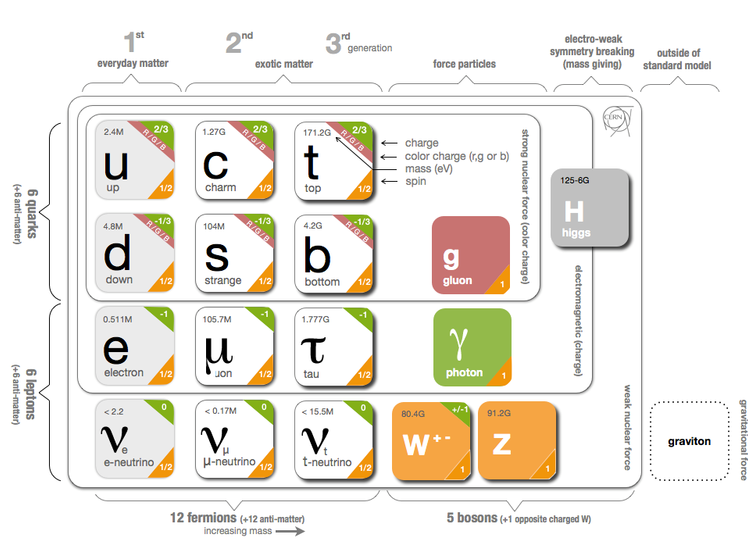
\includegraphics[width=0.8\linewidth]{SM.png}
			\caption{The Standard Model contents, source \cite{SM}. \label{fig:SM}}
		\end{figure} 
	\end{frame}
	\note{
		SM explain with great precision- fundamental particles in figure w/ charge, spin and mass - 17 particles - fermions and bosons.
		Does not explain graviton - non-zero mass of neutrino. Know from neutrino oscillations from the Sun - they change flavor and must have mass.
		
		Introduce Inverse seesaw mechanism w/ heavy neutrinos and right-handed neutrinos. Only left-handed neutrinos, LH and RH for other SM particles. LH means direction of spin and motion are opposite. ISS-> trilepton final state with a neutrino through p-p collisions and decay through W-boson and heavy pseudo-Dirac neutrino. Continue to next slide with model->
	}


	\begin{frame}[t]{Trilepton Final State}
		\begin{figure}[htbp!]
			\centering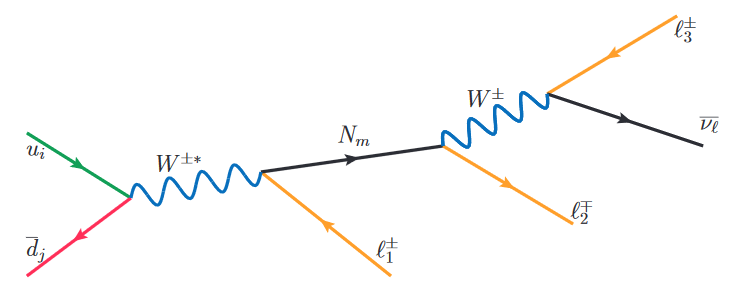
\includegraphics[width=0.8\linewidth]{ModelProcess.png}
			\caption{The Born diagram for the charged current Drell-Yan process of the proton-proton collision (on the left) producing a heavy pseudo-Dirac neutrino $N$ in the inverse seesaw mechanism model, leading to a trilepton plus missing transverse energy (a light neutrino) final state. Figure is taken from ref. \citet{inverseseesaw}. \label{fig:ModelProcessIntro}}
		\end{figure}
	\end{frame}
	\note{
		Figure of P-P collisions to trilepton final state and decays. Charges. At LHC and CERN, detected by ATLAS but neutrinos are not. Only MET since conservation of energy.
		
		Called charged current Drell-Yan process, same model we look at for neutrinos as by \citet{inverseseesaw}. Gives almost conserved lepton number and consider only electrons and muons. Amount of SS and OS events vertex 1 and 2 differ from normal seesaw. Allows LFV for vertex 1 and 2 for e and mu. Study two simulated neutrino signals, mass 150 GeV and 450 GeV, expect different LFV for different neutrino mass models.
	}


	\begin{frame}[t]{Lepton Flavor Distributions}
		\begin{figure}[htbp!]
			\hspace*{-1.0cm}
			\centering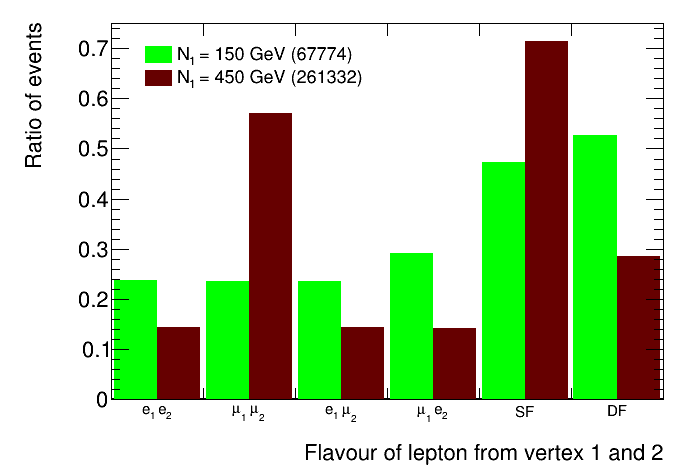
\includegraphics[width=0.8\linewidth]{h_sf_df_dist_truth.png}
			\caption[Lepton flavor distribution between vertex 1 and 2.]{Distribution of the lepton flavor between vertex 1 and 2 for the 150 and 450 GeV signals where we either have two electrons, or two muons (SF) or an electron and a muon (DF).  \label{fig:LepFlavDist}}
		\end{figure} 
	\end{frame}
	\note{
		Distributions of lepton flavor - event ratios lepton 1 and 2 - electrons and muons - two neutrino signals - SF: ee or mumu - DF: emu or mue. 450 - more SF events - 150 - barely more DF events.
	}


	\begin{frame}[t]{Proton-Proton Collision Data}
		\begin{figure}[htb!]
			\hspace*{-0.6cm}
			\centering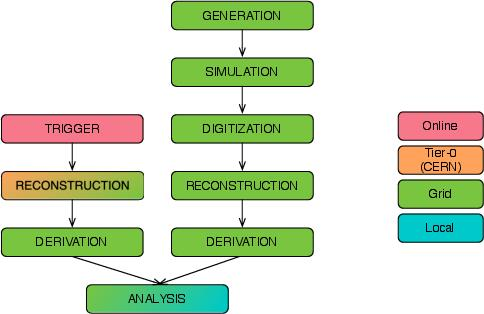
\includegraphics[width=0.8\linewidth]{dataFlow.png}
			\caption{The data flow for producing the proton-proton collision data and simulations. Credit: \citet{catmore2020atlas}. \label{fig:DataFlow}}
		\end{figure}
	\end{frame}
	\note{
		MC simulated backgrounds, simulated neutrinos and p-p data at 13 TeV from LHC 2018 - data flow left side - not interesting. MC and signals - right side - ML. 
		
		Signal sim - train ML - after Generation - truth. MC - best represent all prod-mech with trilepton+MET. MC + signals - classif after Analysis.
	}


	\begin{frame}[t]{Data Features}
		Original dataset features:
		\begin{itemize}
			\item Flavor, Charge, $\eta$, $\phi$, $p_T$, $E_T^{miss}$.
		\end{itemize}
		New and added features:
		\begin{itemize}
			\item $p_x$, $p_y$, $p_z$, $\theta$, $E$.
			\item $\Delta\phi$, $\Delta R$, $m_{ll}$, $m_{3l}$.
		\end{itemize}
		Target features:
		\begin{itemize}
			\item $[123, 132, 213, 231, 312, 321]$
		\end{itemize}
	\end{frame}
	\note{
		Not always trivial to identify particles. P-P collisions simulated, and measure properties like momentum, transverse momentum and coord-angles. Make new variables dPhi, dR and mll, m3l.
		
		Make target classes - vertex permutations - three vertices, model in slide 4. Leading, subleading, subsubleading - wrt. pT - leading lepton = lepton 1, highest pT - six possible permutations to classify w/ML.
	}


	\begin{frame}[t]{Feature Distributions}
		\begin{figure}[h]
			\centering
			\subfloat{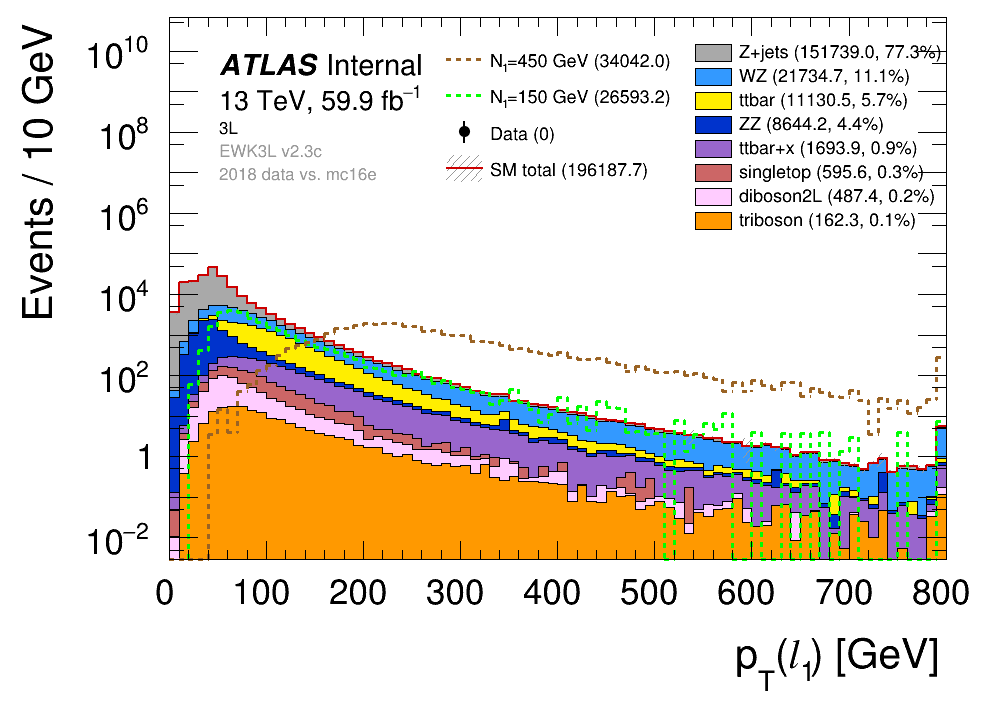
\includegraphics[width=0.5\textwidth]{Feature_plots/hist1d_lep1_pt_3L.png}}
			\subfloat{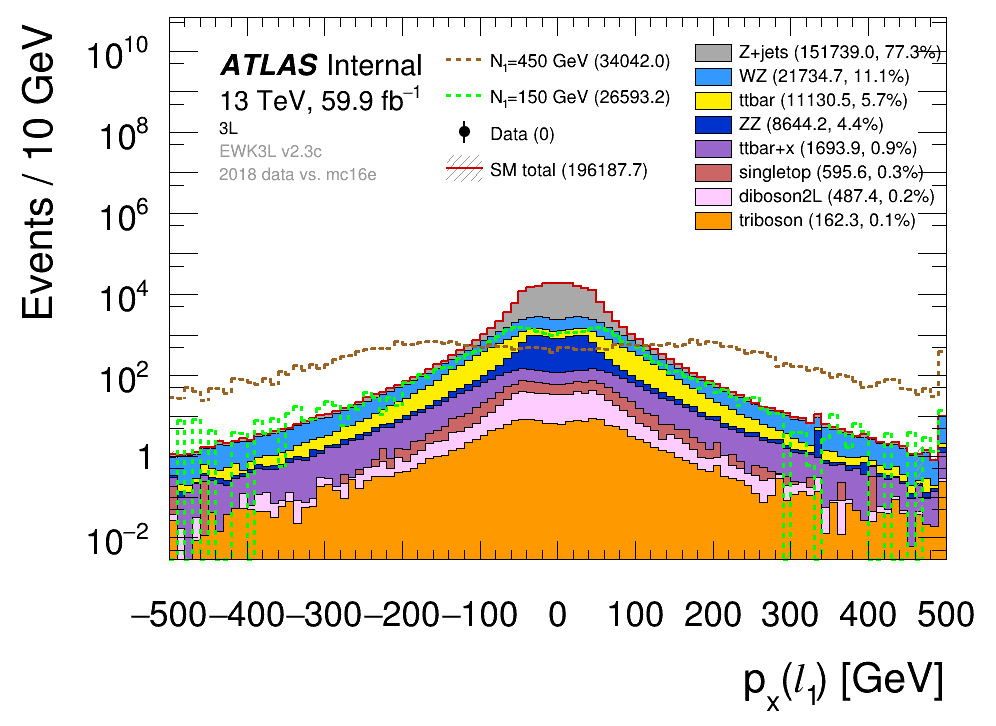
\includegraphics[width=0.5\textwidth]{Feature_plots/hist1d_lep1_px_3L.png}}\\
			\centering
			\subfloat{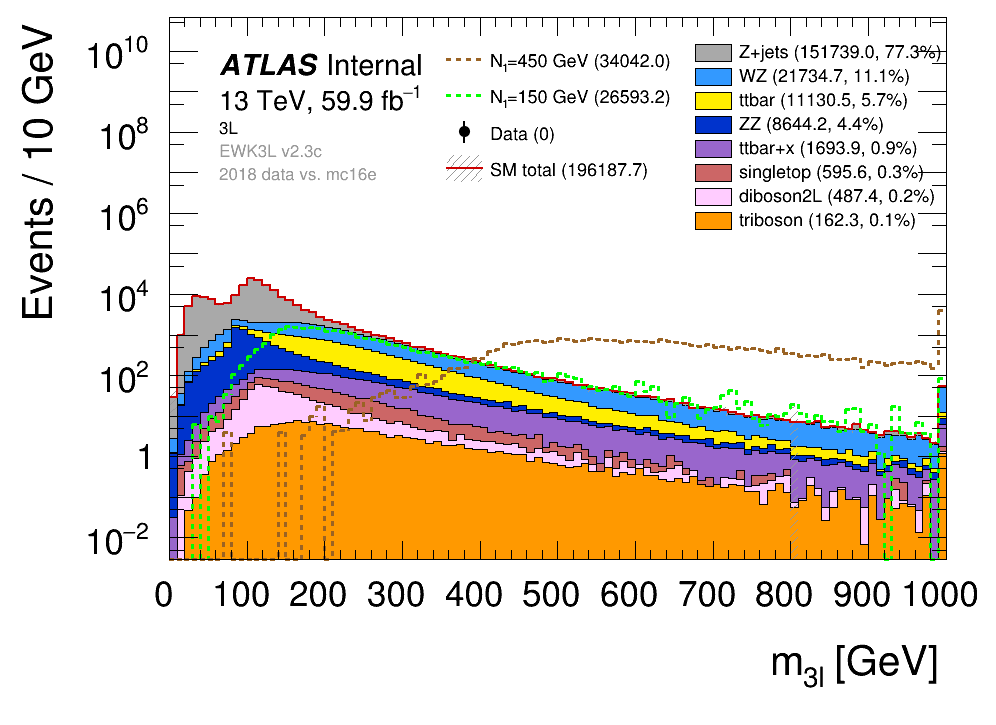
\includegraphics[width=0.5\textwidth]{Feature_plots/hist1d_m_3l_3L.png}}
			\subfloat{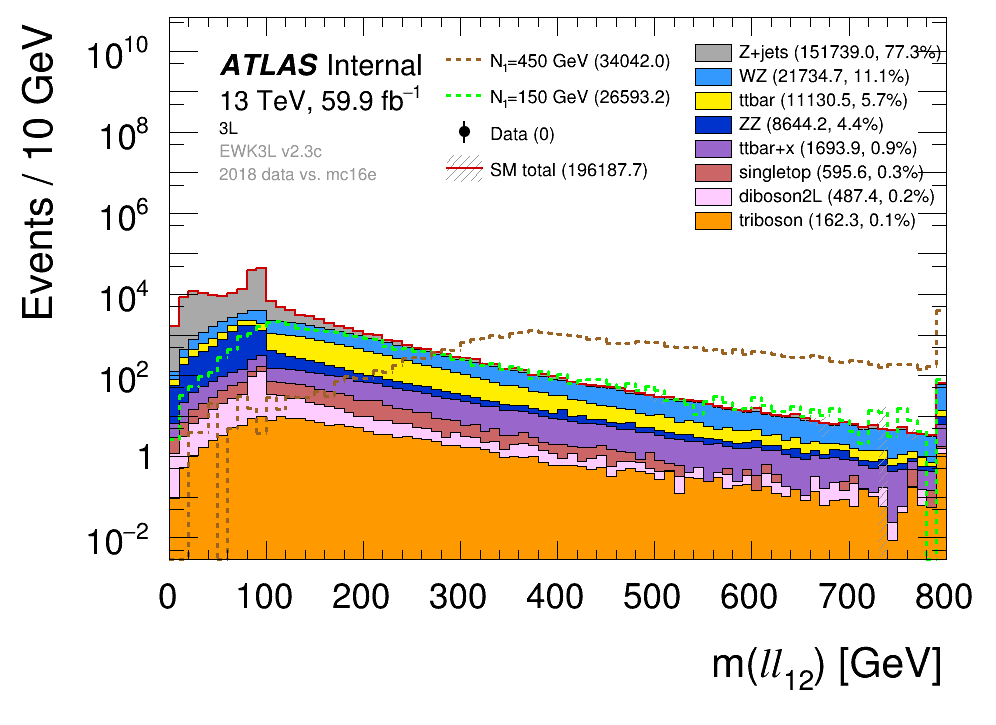
\includegraphics[width=0.5\textwidth]{Feature_plots/hist1d_mll_12_3L.png}}
		\end{figure}
	\end{frame}


	\begin{frame}[t]{*Machine Learning Process}
		\begin{block}{What we want to do:}
			Use machine learning to identify lepton vertices in simulated backgrounds and signals.
		\end{block}
		\begin{block}{How to do it:}
			\begin{enumerate}[I]
				\item Use supervised learning and multiclass classification.
				\item Train and optimize machine learning algorithms
				\item Evaluate which model that best predicts the vertices.
				\item Predict lepton vertices for simulated backgrounds and signals.
			\end{enumerate}
		\end{block}
		\begin{block}{End goal:}
			\begin{enumerate}[I]
				\item Look for lepton flavor violation between the classified leptons 1 and 2.
				\item Compare with a more standard analysis by \citet{inverseseesaw}.
			\end{enumerate}
		\end{block}
	\end{frame}
	\note{
		Machine learning to train to identify the particles vertices, pattern recognition in particle properties. Truth simulated data, know the origins and what particles have been produced. Train various ML algorithms, use best performing model to predict simulated backgrounds and signals. Six different lepton vertex permutations. Multiclass classification case with six classes, not been studied much previously in particle physics. 
		
		Need good and fast algorithms for classification, lot of data to work with. Need preprocessing of data before classification. Train models on training set. Many hyperparameters to optimize on validation set. Evaluation metrics for performance evaluation for validation and test set. Export best model, skips training the models each time.
		
		Signal region cuts to study LFV for lepton 1 and 2. Compare with a more standard analysis by \citet{inverseseesaw}.
	}


	\begin{frame}[t]{Preprocessing of Data}
		\begin{enumerate}[(i)]
			\item Feature correlations
			\item Resampling
			\item Splitting into data sets
			\item Scaling
		\end{enumerate}
	\end{frame}
	\note{
		Check correlations - strong correlations=strong linear dependence=remove one feature=should give better results. Information gain - want higher values=features have more information regarding the classes.
		
		Imbalanced data=more data for some classes (bias)=bad predictions of minority classes - resampling techniques to balance classes (number of events).
		
		Split data - training, validation, test - training=train models - validation=tune model hyperparameters and check models - test=check final performance of (tuned) models.
		
		Scale - avoid weighted favoring of some classes - only for features - standardization=0 mean, 1 std.dev.
		
		Tune with a randomized search method with cross-validation for different hyperparameters depending on classification type and algorithm. 
	}


	\begin{frame}[t]{Bias-Variance Tradeoff}
		\begin{figure}[htbp!]
			\centering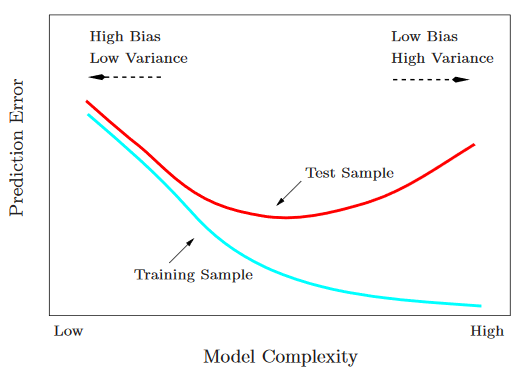
\includegraphics[width=0.8\linewidth]{bias-variance.png}
			\caption{Illustration of the quality of a model from how well it does on data not seen during training with variance and bias regions. Source by \citet{mehta2019high}. \label{fig:BiasVar}}
		\end{figure}
	\end{frame}
	\note{
		Supervised learning problem - balance between variance and bias - best compromise=best model for model complexity/number of data points. High bias=underfitting - high variance=overfitting. Overfitting more normal today. Figure - optimal at test minimum. Quality of model - on data not seen during training.
	}


	\begin{frame}[t]{Classification Algorithms}
		Types of classification algorithms used:
		\begin{enumerate}[(i)]
			\item Logistic regression
			\item Multi-layer perceptron
			\item Trees
			\item Boosters
			\item Multiclassifiers
		\end{enumerate}
	\end{frame}
	\note{
		Binary classifiers to multiclass: LR - linear regression with a logistic function to predict. MLP - neural network - input, hidden, output layers - weights, biases, non-linear activation func to output - hyperparameters, regularization control overfitting. DTC - simpler, single tree model with features - criterion for value splits - control hyperparm for overfit. RF - ensemble of trees - increase accuracy, decease variance. Boost - iteration weights - sequential models built - better classifier. AdaBoost - adaptive boost - weights adapt each iteration - majority vote -> better classifier. GradientBoost - tree boost approx Ada - weighted gradient in loss func - HistGradient larger data sets - less time, higher accuracy - bins. XGB - opt hist dist grad boost alg - accurate fast parallel - scalable -  dist of features - complex w/hyperparameters. LGBM - distributed gradient boost - faster, memory efficient, accurate - large data sets - information gain - drop feat threshold.
		
		Multiclass: Multiclass to binary cases techniques.
	}


	\begin{frame}[t]{Classification Results}
		\begin{table}[htbp!]
			\centering
			%\hspace{-1cm}
			\begin{tabular}{ |c|c|c|c|c| }
				\hline \rule{0pt}{13pt}
				\multirow{2}{*}{Model} & \multicolumn{4}{c|}{Signal models} \\
				\cline{2-5} \rule{0pt}{13pt}
				 & \multicolumn{2}{c|}{150 GeV} & \multicolumn{2}{c|}{450 GeV} \\
				\cline{2-5} \rule{0pt}{13pt}
				 & Score & Score\_train & Score & Score\_train \\
				\hline \rule{0pt}{13pt}
				AdaBoost & 0.8519 & 1.0000 & 0.9385 & 1.0000 \\
				\hline \rule{0pt}{13pt}
				OvO & 0.7788 & 0.9299 & 0.9088 & 0.9319 \\
				\hline \rule{0pt}{13pt}
				MLP & 0.8227 & 0.9492 & 0.9350 & 0.9606 \\
				\hline \rule{0pt}{13pt}
				HGBC & 0.7863 & 0.8999 & 0.9280 & 0.9571 \\
				\hline \rule{0pt}{13pt}
				XGBoost & 0.8631 & 0.9998 & 0.9509 & 0.9999 \\
				\hline \rule{0pt}{13pt}
				LGBM & \textbf{0.8779} & 0.9999 & \textbf{0.9541} & 0.9999\\
				\hline
			\end{tabular}	
			\caption{Accuracy scores of the highest performing classification models trained on the 150 GeV and 450 GeV validation and training sets.}
			\label{tab:Validation}
		\end{table}
	\end{frame}
	\note{
		Highest scoring - both signals - validation and training scores. Tendency to overfit - 450 scores closer. XGB and LGBM best - LGBM better and faster - LGBM chosen.
	}


	\begin{frame}[t]{Light Gradient Boosting Machine}
		\begin{figure}[h]
			\centering
			\subfloat{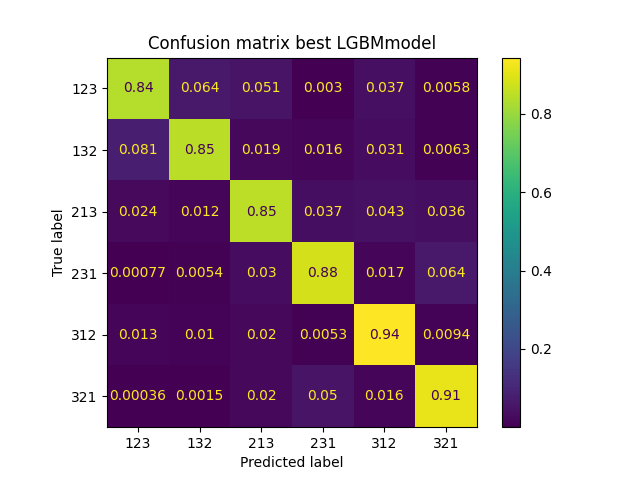
\includegraphics[width=0.5\textwidth]{Test_plots/Conf_mat_150.png}}
			\subfloat{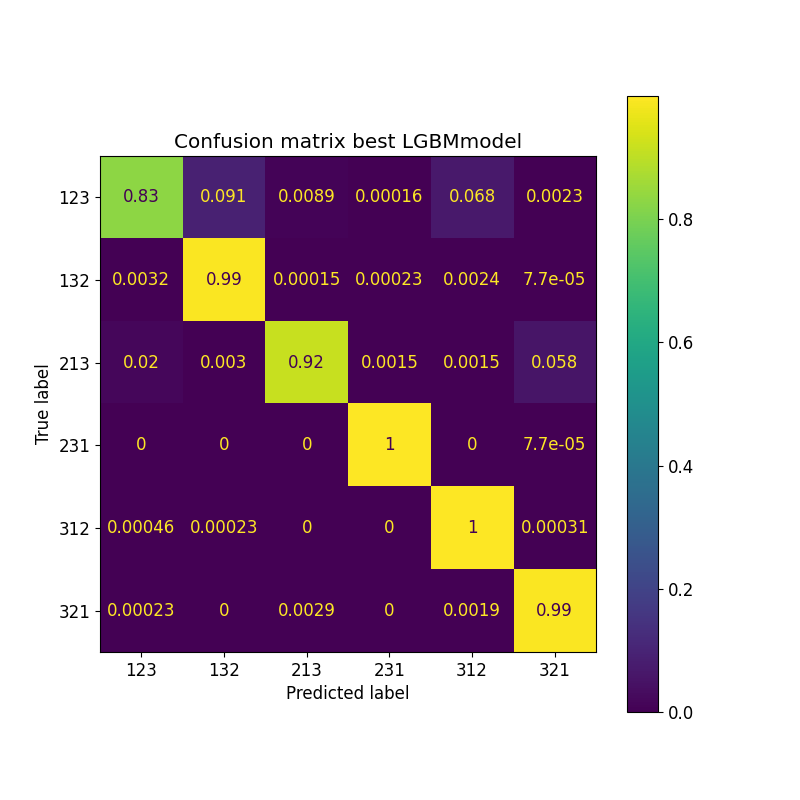
\includegraphics[width=0.5\textwidth]{Test_plots/Conf_mat_450.png}}
			\caption{Light Gradient Boosting Mechanism (LGBM) confusion matrix on the test set for both signals.}
		\end{figure}
	\end{frame}
	\note{
		LGBM on test data - no tuning - more metrics. Confusion matrices - diagonal between 0.8-1.0 - good predictions. 450 GeV more accurate - 132, 231, 312, 321 better accuracy.
	}


	\begin{frame}[t]{Scores}
		\begin{table}[htb!]
			%\hspace{-0.8cm}
			\centering
			\begin{tabular}{ |c|c|c|c|c| }
				\hline \rule{0pt}{13pt}
				Signal [GeV] & Score & Score\_train & CKS & LogLoss  \\
				\hline \rule{0pt}{13pt}
				150 & 0.8793 & 0.9999 & 0.8551 & 0.3335 \\
				\hline \rule{0pt}{13pt}
				450 & 0.9570 & 0.9999 & 0.9484 & 0.1120 \\
				\hline
			\end{tabular}	         
			\caption{Accuracy score of both the test and training sets, Cohen Kappe score and logloss for both the 150 and 450 GeV signal models.}
			\label{tab:Test}
		\end{table}
		\begin{table}[htb!]
			%\hspace{-0.8cm}
			\centering
			\begin{tabular}{ |c|c|c|c| }
				\hline \rule{0pt}{13pt}
				\multirow{2}{*}{Signal [GeV]} & \multicolumn{2}{c|}{ROC} & \multicolumn{1}{c|}{Precision-Recall}\\
				\cline{2-4} \rule{0pt}{13pt}
				 & Micro AUC & Macro AUC & Micro AUC  \\
				\hline \rule{0pt}{13pt}
				150 & 0.99 & 0.99 & 0.949 \\
				\hline \rule{0pt}{13pt}
				450 & 1.0 & 1.0 & 0.994  \\
				\hline
			\end{tabular}	         
			\caption{Micro and macro area under the curve (AUC) scores for both ROC and precision-recall curves.}
			\label{tab:AUC}
		\end{table}
	\end{frame}
	\note{
		Table 1: Accuracy scores, CKS and log loss (error) of LGBM - validation and test similar accuracy - good for different data - NB: same original data set. 450 GeV still better - high acc - low log loss.
		
		Table 2: Micro and macro AUC for ROC and precision-recall - show overall performance - AUC over 0.8=good model - both values over 0.9. LGBM shows great promise on predicting the vertices on these test set.
	}


	\begin{frame}[t]{Classify Simulated Data}
		What to classify with the LGBM:
		\begin{enumerate}[(i)]
			\item Simulated background production-mechanisms with trilepton final states plus MET.
			\item Two reconstructed neutrino signals, with neutrino masses of 150 and 450 GeV.
		\end{enumerate}
	
		\begin{itemize}
			\item Use classified vertex permutations to define new signal regions with opposite sign and same flavor or opposite flavor for lepton 1 and 2.
			\item Compare signal regions with benchmark analysis.
		\end{itemize}
	\end{frame}
	\note{
		LGBM - performs well on truth neutrino signals - classify similar datasets - simulated backgrounds and signals - same neutrino masses.
		
		Expected - most events with highest $p_T$ from $N_1$ production - loose momentum after decaying - 123 and 132 vertices most both - few 213 also for MC - enough for further analysis.
	}


	\begin{frame}[t]{Predicted Signal Vertices}
		\begin{figure}[htbp!]
			\centering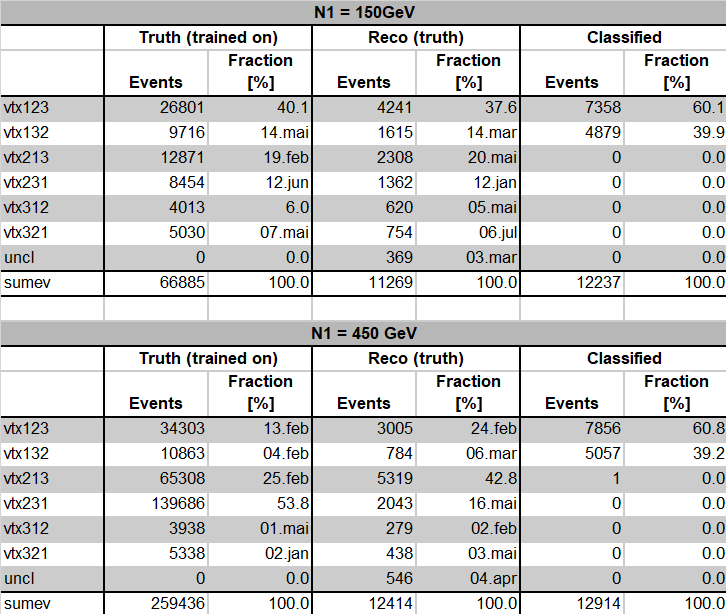
\includegraphics[width=0.7\linewidth]{Signal_table.png}
			\caption{Number of events for each vertex of the two signals and the fraction for each vertex. Left: the truth data we used to train our classifiers on. Middle: The truth vertices for the reconstructed signals we predict. Right: The classified vertices of the reconstructed signals. \label{fig:NeutrinoClass}}
		\end{figure}
	\end{frame}
	\note{
		Extra: Check on signal predictions - see table for vertex events - 150 and 450 predicted with respective model - see number of events for each vertex + fractions. Left: original truth data - training ML - Middle: reconstructed signals we classify - Right: classified vertices.
		
		Interesting to mention - truth after Generation and recon 150 GeV - similar event fractions - 450 GeV have not as close. Events disappears after reconstruction - between left to middle. Classif - 123 and 132 predicted - one 213 with 450 - predictions does not fit truth recon - Why? - LGBM trained on signals before recon in data flow - not sure if true, a guess - further analysis needed?
	}


	\begin{frame}[t]{Signal Regions}
		\begin{itemize}
			\item SF \& OS
			\item DF \& OS
			\item Vertex = [123, 132, 213]
		\end{itemize}
	
		\begin{table}[ht!]
			\centering
			\begin{tabular}{|c|}
				\hline \rule{0pt}{13pt}
				\textbf{Benchmark "Standard" Analysis at $\sqrt{s}=$ 14 TeV:}\\
				\hline \rule{0pt}{13pt}
				$m_{l_i,l_j}>$ 10 GeV,\quad $|m_{l_i,l_j}-M_Z|>$ 15 GeV,\quad $|m_{3l}-M_Z|>$ 15 GeV,\\
				$p_T^{l_1}>$ 55 GeV,\quad $p_T^{l_2}>$ 15 GeV,\quad $m_{3l}>$ 80 GeV\\
				\hline
			\end{tabular}
			\caption{Cuts used for a benchmark analysis. The combinations of $l_il_j$ are for $l_1$, $l_2$ and $l_3$. $M_Z=91.2$ GeV is the mass of the $Z$-boson and $m_{3l}$ is the invariant mass of the three lepton system. Reference: Table 6 in \citet{inverseseesaw}.}
			\label{tab:Cuts_Benchmark}
		\end{table}
	\end{frame}
	\note{
		SF, DF and OS between classified lepton 1 and 2.
		
		Compare with standard analysis - missing one b-tagged cut - not available in datasets.
	}


	\begin{frame}[t]{Analysis Results}
		Look at:
		\begin{itemize}
			\item Invariant mass of three lepton system, $m_{3l}$, and MET (neutrino).
			\item Event distributions and significance.
			\item SF versus DF.
			\item ML versus benchmark.
		\end{itemize}
	\end{frame}
	\note{
		Invariant mass three lepton system and MET - event distributions and significance - high significance=high sensitivity - where to cut on variable to maximize sensitivity.
		
		Much less events after cuts - more events for SF - difference from Z not decaying into electron-muon events - less events for large MC (DF) like WZ and Z+jets - same number events for signals SF and DF.
		
		213 - no significance, no signal - few MC events - little information from 213 distributions here.
		
		450 GeV sim signal - easier to differentiate with MC - masses above 400-500 GeV for $m_{3l}$ - somewhat visible for MET at 100-400 GeV - MET does not discriminate well signals and MC, as expected.
		
		Significance higher for 450 GeV comp 150 GeV - higher for $m_{3l}$ comp MET. Our model better than the benchmark.
	}


	\begin{frame}[t]{Summary and Outlook}
		\begin{itemize}
			\item We have shown that multiclass classification is well suited for predicting from which vertex a lepton comes from.
			\item Proper data is a challenge to avoid overfitting and bad predictions. Preprocessing of data and tuning hyperparameters needed.
			\item Different number of events for SF and DF.
			\item Trained multiclass model performs better than benchmark model.
		\end{itemize}
	
		Modern ML techniques are rapidly modified and developed in the field of particle physics and high energy physics analysis.
	\end{frame}
	\note{
		Shown - use multiclass classification and ML - predict and classify - sim of subseq decay leptons - from p-p collisions - final state model w/three leptons + neutrino.
		
		Training models - proper data - big challenge - overfitting and bad predictions. Preprocessing data - tuning hyperparameters.
		
		Lepton Flavor violation - SF more events - lep 1 and 2 - predicted vertices - high significance in some signal regions. 
		
		ML models better than benchmark - benchmark not optimized.
		
		Future: Modern ML techniques - modified and developed - particle physics and HEP analysis - better suited model to test. Other particle aspects future - other neutrino masses - SS vs OS - include detector data from CERN.
	}

	
%--------------
	\begin{frame}[t]{References}
		\bibliographystyle{unsrtnat} %plain, unsrt, abbrv
		\bibliography{Refs}
	\end{frame}

\end{document}